\section{Vector Bundles}

\begin{definition}
    Let $M$ be a \underline{topological space}. A \emph{real vector bundle of rank $k$ over $M$} is a topological space $E$ together with a continuous surjection $\pi: E\onto M$ satisfying the following conditions: 
    \begin{enumerate}[label=(\alph*)]
        \item For each $p\in M$, the fiber $E_p = \pi^{-1}(p)$ over $p$ is endowed with the structure of a $k$-dimensional real vector space.
        \item For every $p\in M$, there is a neighborhood $U$ of $p$ in $M$ and a homeomorophism $\Phi:\pi^{-1}(U)\to U\times\R^k$, called a \emph{local trivialization of $E$ over $U$} satisfying the following additional conditions: 
        \begin{itemize}
            \item If $\pi_U: U\times\R^k\onto U$ is the natural projection, then $\pi_U\circ\Phi = \pi$.
            \item For each $q\in U$, the restriction of $\Phi$ to $E_q$ is a vector space isomorphism from $E_q$ to $\{q\}\times\R^k\cong\R^k$.
        \end{itemize}
    \end{enumerate}
\end{definition}

\begin{figure}[H]\label{fig:vector-bundle-illustration}
    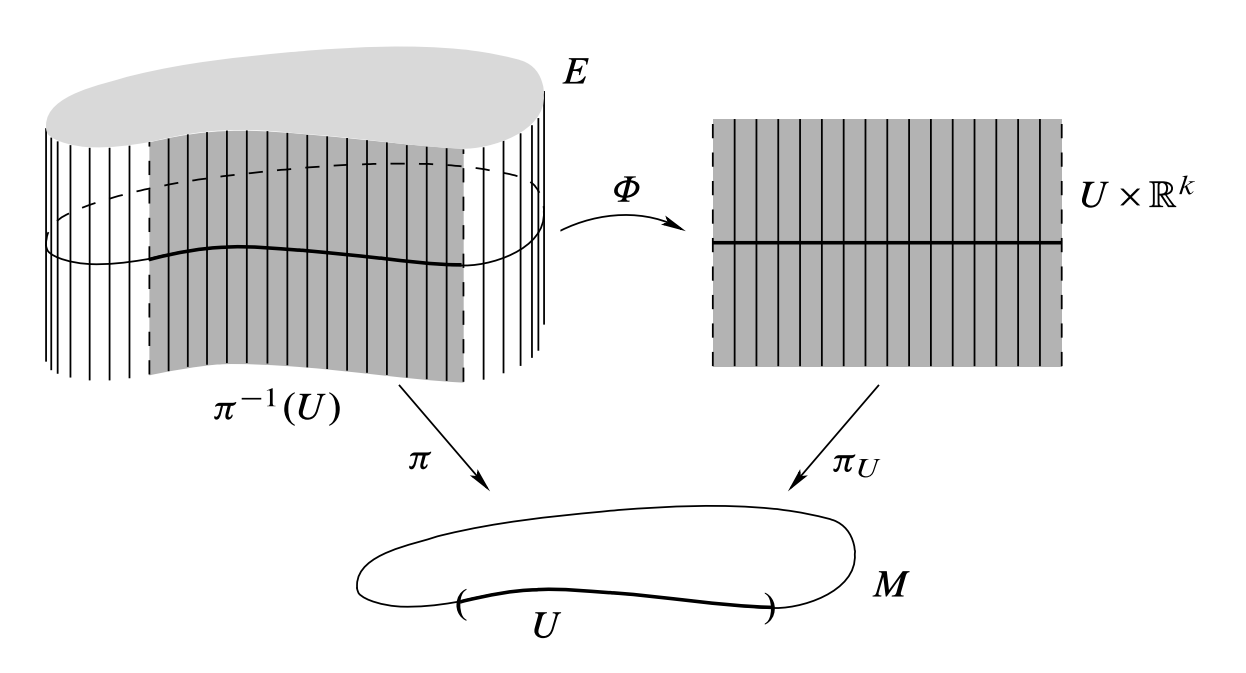
\includegraphics[width=\textwidth, height=0.3\textheight]{images/vector-bundle-illustration.png}
    \caption{A local trivialization of a vector Bundle}
\end{figure}